%%%%%%%%%%%%%%%%%%%%%%%%%%%%%%%%%%%%%%%%%%%%%%%%%%%%%%%%%%%%%%%%%
%  _____   ____  _____                                          %
% |_   _| /  __||  __ \    Institute of Computitional Physics   %
%   | |  |  /   | |__) |   Zuercher Hochschule Winterthur       %
%   | |  | (    |  ___/    (University of Applied Sciences)     %
%  _| |_ |  \__ | |        8401 Winterthur, Switzerland         %
% |_____| \____||_|                                             %
%%%%%%%%%%%%%%%%%%%%%%%%%%%%%%%%%%%%%%%%%%%%%%%%%%%%%%%%%%%%%%%%%
%
% Project     : LaTeX doc Vorlage für Windows ProTeXt mit TexMakerX
% Title       : 
% File        : grundlagen.tex Rev. 00
% Date        : 7.5.12
% Author      : Remo Ritzmann
% Feedback bitte an Email: remo.ritzmann@pfunzle.ch
%
%%%%%%%%%%%%%%%%%%%%%%%%%%%%%%%%%%%%%%%%%%%%%%%%%%%%%%%%%%%%%%%%%

\chapter{Technical Foundation}\label{chap.grundlagen}
\section{Reinforcement Learning}\label{reinforcementlearning}
\subsection*{Basic Definitions}\label{basic_rl_definitions}
In recent years, major progress has been achieved in the field of reinforcement learning (RL) \cite{mnih2013playing},\cite{alphazero}, \cite{hideandseek}.
In RL, an agent $\mathcal{A}$ learns to perform a task by interacting with an environment $\mathcal{E}$. On every timestep $\mathcal{t}$ the agent needs to take an action $\mathcal{u}$. The selection of this action $\mathcal{u}$ is based on the current observation $\mathcal{s}$. The success of the agent is measured by reward $\mathcal{R}$ received. If the agent does well, it receives positive reward from the environment, if it does something bad, there is no or negative reward. The goal of the agent $\mathcal{A}$ is now to take an action that maximizes the expected future reward  $\EX[\mathcal{R}_{t+1}+\mathcal{R}_{t+1}+\mathcal{R}_{t+1}+...|\mathcal{s}_{t}]$ given the current observation $\mathcal{s}$.\\
The current observation $\mathcal{s}_{t}$, also known as the current state is used to determine which action $\mathcal{u}$ to take next. An agent can observe its environment either fully or partially.


\subsection*{Value Based vs. Policy Gradient Based Methods}\label{value_policy_based_methods}
Reinforcement learning methods are categorized into value-based methods and policy-based methods\cite{tdlearning},\cite{policygradient}. Those variants differ on how they select an action $\mathcal{u}$ from a state $\mathcal{s}$.
Value-based RL algorithms work by learning a value function $\mathcal{V(s)}$ through repeated rollouts of the environment. $\mathcal{V(s)}$ aims to estimate the future expected reward for any given state $\mathcal{s}$ as precisely as possible. Using this approximation $\mathcal{V(s)}$ we can now select the action $\mathcal{u}$ that takes the agent into the next state $\mathcal{s}_{t+1}$ with the highest expected future reward. This estimation $\mathcal{V(s)}$ is achieved by either a lookup table for all possible states or a function approximator. In this work, we solely focus on the case that $\mathcal{V(s)}$ is implemented in form of a neural network as function approximator.\\
The second category of reinfocement learning algrithms are the so called policy gradient based methods. These methods aim to aquire a stochastic policy $\pi$ that maximizes the expected future reward $\mathcal{R}$ by taking actions with certain probabilities. Taking actions based on probabilities solves an important issue of value based methods, which is, that by taking greedy actions with respect to state  $\mathcal{s}$, the agent might not explore the whole state space and misses out on better ways to act in the environment.


\subsection*{Asynchronous advantage actor critic algorithm}\label{a3c_intro}
The progress in RL has led to algorithms that combine value based and policy gradient based methods. To enhance the process of learning policy $\pi$, the policy loss gets multiplied by the difference between actually received reward $\mathcal{R}$ and the estimated future reward $\mathcal{V(s)}$. 
TODO: Extend


\subsection*{Relation to this Work}\label{rl_relation_work}
The goal of this work is to apply an RL algorithm to the vehicle rescheduling problem. Based on the work of S. Hubacher (source!!!), we use a distributed RL algorithm that learns a policy to control the traffic of trains on a rail grid. To do so, we use the asynchronous advantage actor critic algorithm \cite{a3c} and expand its definiton to the use case of multiple agents, similar to \cite{marltraffica3c}.

\section{The Flatland Rail Environment}\label{projektmanagement}
The flatland environment is a virtual simulation environment provided by the Swiss Federal Railway SBB and the crowdsourcing platform AICrowd.
The goal of this environment is to act as a simplified simulation of real train traffic. Using flatland, we can train RL algrithms to control the actions of trains, based on observations on the grid. Flatland has a discrete structure in both its positions and its timesteps.The whole rail grid is composed out of squares that can have connections to neighbouring squares. In certain squares, the rails splits into two rails. On those switches, the agent has to make a decision which action it wants to take. Dependent on the type of switch, there are different actions available. All rail parts, independent of if it is a switch also allow to take the actions to do nothing (remain halted, or keep driving), to go forward or to brake. 
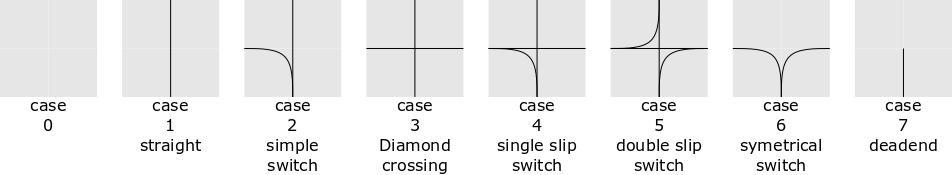
\includegraphics[width=0.7\textwidth, height=30px]{images/transition_nips_proposal.png}
The action space is therefore defined by:
\begin{gather*}
U = \{ \text{Do nothing, go left, go forward, go right, brake} \}
\end{gather*}
It is important to note that trains do not have the ability to go backwards and therefore need to plan ahead to avoid getting stuck. To learn which actions to take, the agents have to learn to adapt to an unknown environment due to the fact that the environments are randomly generated and differ on each episode. Depending on the given parameters, the size and complexity of the grid can be adjusted. This allows for dynamically changing the difficulty for the agents.\\
The goal of each agent is to reach an assigned target train station as fast as possible. Agents that reach this destination are removed from the grid which means, they can no longer obstruct the path of other trains.
\subsection*{Agent Evaluation}\label{rl_agent_eval}
AICrowd an SBB provide a system for agent evaluation. This system evaluates the policy on a number of unknown environments and outputs the percentage of agents that reached their destination as well as the received reward while doing so. The evaluation reward scheme is thereby as follows:
\begin{gather*}
R_{t}= 
\begin{cases}
-1,				& \text{if } s_{t} \text{ is not terminal}\\
10,             & \text{otherwise}
\end{cases}
\end{gather*}
All submissions to the flatland challenge are getting graded by the percentage of agents that made it to destionation. (Source) Additionally we use our own evaluation parcour with an increasing difficulty of environments to get more insight into the agents strenghts and weaknesses.
\subsection*{Observations}\label{observations}
The flatland environment allows to create observation builders to observe the environment for each agent. While it is possible to observe the whole grid, this does usually not make sense due to the fact that many parts of the rail grid are not relevant to a single train. Flatland offers by default two different observation builders.\\
\textbf{GlobalObsForRailEnv} creates three arrays with the dimensions of the rectangular rail grid. The first array contains the transition information of the rail grid. For each cells, there are 16 bit values, 4 for each possible direction a train is facing.
\textbf{TreeObsForRailEnv} creates a graph with sections of the grid as nodes from the perspective of the train.
This means, only the switches which the train is actually able to take define a single node.

